\documentclass[12pt]{article}
\usepackage[margin=1in]{geometry}
\usepackage[all]{xy}

\usepackage{amsmath,amsthm,amssymb,color,latexsym,soul}
\usepackage{geometry}        
\geometry{letterpaper}    
\usepackage{graphicx}
\usepackage{enumitem}
\usepackage{listings}
\usepackage{xcolor}
\usepackage{bm}

\definecolor{codegreen}{rgb}{0,0.6,0}
\definecolor{codegray}{rgb}{0.5,0.5,0.5}
\definecolor{codepurple}{rgb}{0.58,0,0.82}
\definecolor{backcolour}{rgb}{0.95,0.95,0.92}

\lstdefinestyle{mystyle}{ % taken from: https://www.overleaf.com/learn/latex/Code_listing
    backgroundcolor=\color{backcolour},   
    commentstyle=\color{codegreen},
    keywordstyle=\color{magenta},
    numberstyle=\tiny\color{codegray},
    stringstyle=\color{codepurple},
    basicstyle=\ttfamily\footnotesize,
    % breakatwhitespace=false,         
    breaklines=true,                 
    captionpos=b,                    
    keepspaces=true,                 
    % numbers=left,                    
    numbersep=5pt,                  
    % showspaces=false,                
    % showstringspaces=false,
    % showtabs=false,                  
    % tabsize=2
}

\lstset{style=mystyle}

\newtheorem{task}{Task}
\newenvironment{solution}[1][\it{Solution}]{\textbf{#1. } }{$\square$}
\newtheorem{subtask}{\; \; \it{Part}}


\begin{document}
\noindent Asaad Mohammedsaleh \hfill CS249 Assignment 2\\
KAUST Spring 2025 \hfill Genome Assembly and Evaluation


\hrulefill


\section{Task 1.1 De Bruijn Graph (DBG) Assembly}

Requirements of this algorithm are:
\begin{itemize}
    \item Takes FASTQ files as input
    \item Constructs a de Bruijn graph from k-mers (with user-defined k)
    \item Identifies contigs by finding Eulerian paths
    \item Outputs contigs as a FASTA file
\end{itemize}

The implementation of the algorithm can be found in \texttt{src/dbg.go} file. The main function to handle the algorithm's components is \texttt{DBGAssembler}.
Then, there are two helper functions: \texttt{constructDeBruijnGraph} and \texttt{walkGraph}.

\texttt{constructDeBruijnGraph} constructs the de Bruijn graph from the reads. It first creates a map of k-mers to their nodes. Then, it adds the edges to the graph. The graph is represented as a map of k-mers to their nodes, where each node is a struct with the k-mer string, its outgoing edges (a map of other k-mers to the number of times they appear in the reads), and its incoming edges (a map of other k-mers to the number of times they appear in the reads).

\texttt{walkGraph} looks at nodes with no incoming edges and picks the longest outgoing edge, which would be a greedy approach on the most occurence of the k-mer. It then follows the edge to the next node and repeats the process until it reaches a node with no outgoing edges. It then adds the collected contig from this path to the list of contigs. It repeats this process for all nodes with no incoming edges, so essentially the output has the same number of contigs as the number of nodes with no incoming edges.

\texttt{DBGAssembler} then writes the contigs to a FASTA file.

\section{Task 1.2 Overlap-Layout-Consensus (OLC) Assembly}

Requirements of this algorithm are:
\begin{itemize}
    \item Takes FASTQ files as input
    \item Computes all-vs-all read overlaps and constructs an overlap graph,
    using the minimum overlap length n as a parameter
    \item Identifies non-branching paths in the graph
    \item Generates a layout of reads
    \item Computes a consensus sequence for each contig
    \item Outputs contigs as a FASTA file
\end{itemize}

The implementation of the algorithm can be found in \texttt{src/olc.go} file. The main function to handle the algorithm's components is \texttt{OLCAssembler}. Then, there are three helper functions: \texttt{overlap}, \texttt{layout}, and \texttt{consensus}.

\texttt{overlap} computes all-vs-all read overlaps and constructs an overlap graph, using the minimum overlap length \texttt{min\_overlap} as a parameter. It returns a map of reads to their nodes, where each node is a struct with the read string, its outgoing edges (a map of other reads to the largest overlap size), and its incoming edges (a map of other reads to the largest overlap size).
The implementation is a naive approach that iterates over all pairs of reads and checks for overlaps, which worked sufficiently for the assignment's datasets.

\texttt{layout} reduces the size of the overlap graph by removing 1-hop and 2-hop inferrible edges as described in the lecture notes of Johns Hopkins slides \cite{olc_lecture_notes}. During the process, it updates the overlap graph by combining reads that have single in-edges and single out-edges. It then outputs the list of reads of the updated overlap graph as contigs.

\texttt{consensus} is a greedy algorithm that starts from a read with no incoming edges and follows the longest outgoing edge until it reaches a read with no outgoing edges. It then adds the collected contig from this path to the list of contigs. It repeats this process for all reads with no incoming edges, so essentially the output has the same number of contigs as the number of reads with no incoming edges. This is not an optimal solution, but it happened to be a good approximation for the assignment's datasets.



\section{Task 1.3 Applications of assembly algorithms}

\subsection{Task 1.3.1}

\begin{figure}[h]
    \centering
    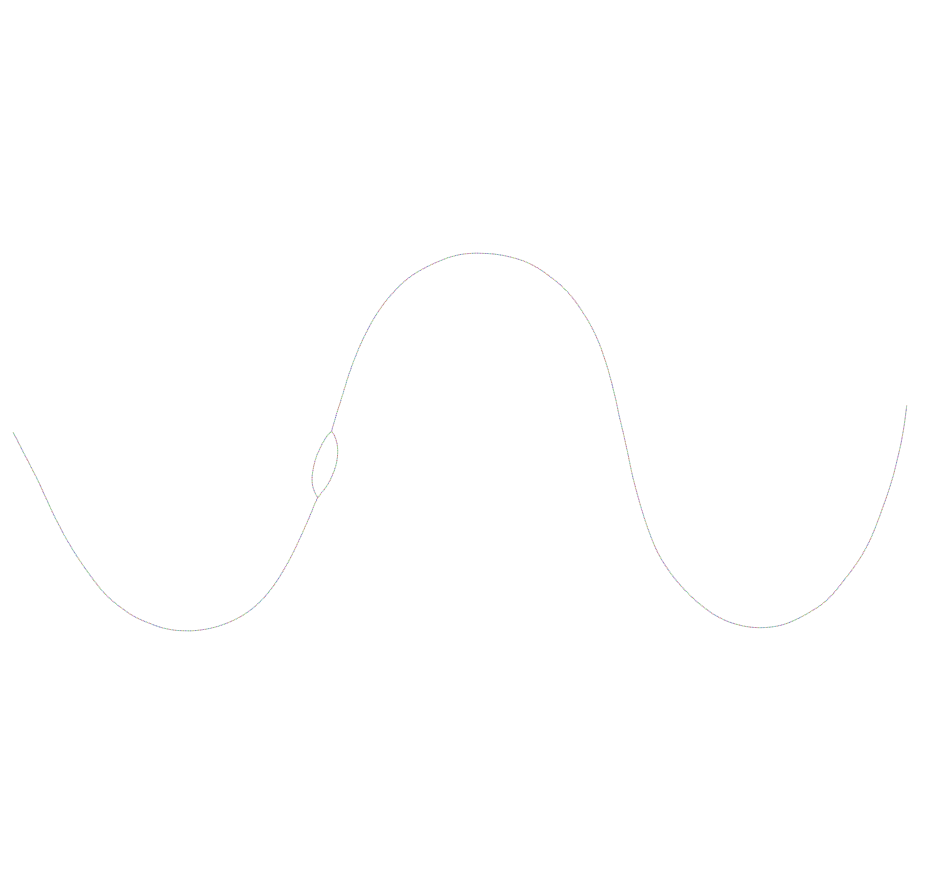
\includegraphics[width=0.5\textwidth]{../toy_dataset/reads_b_k_40.png}
    \caption{Bandage visualization of DBG for k=40}
\end{figure} 

\subsection{Task 1.3.2}

\begin{figure}[h]
    \centering
    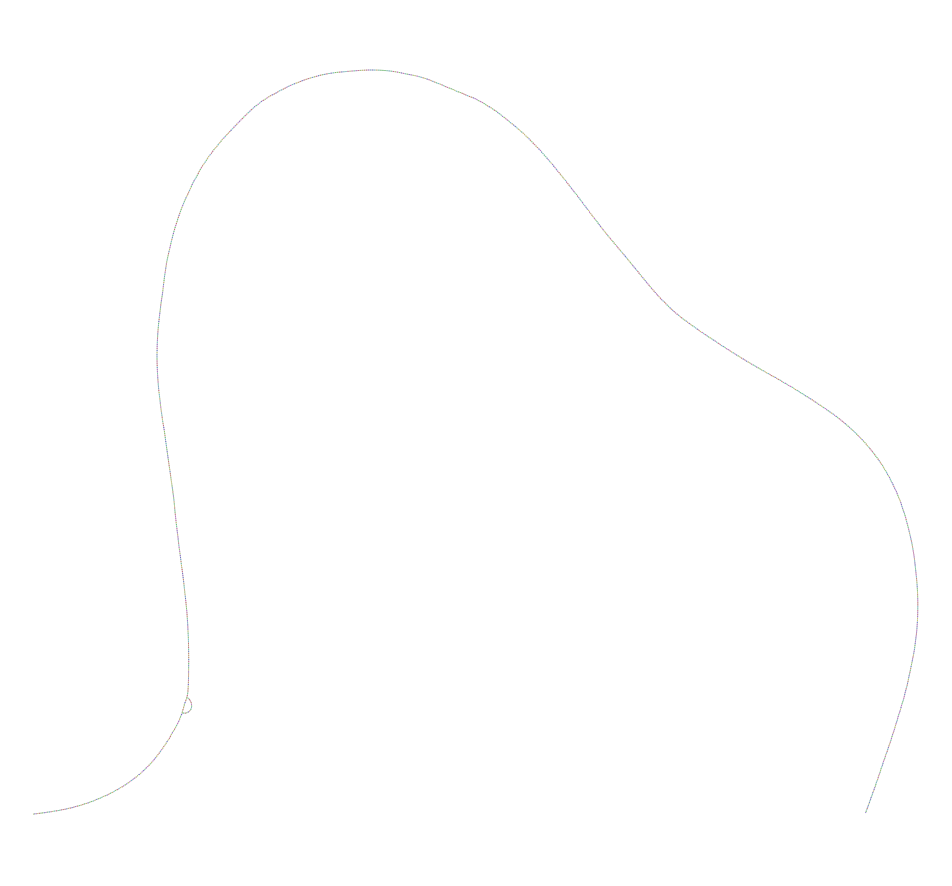
\includegraphics[width=0.5\textwidth]{../toy_dataset/r-k-35.png}
    \caption{Bandage visualization of DBG contigs for k=35 on reads\_r.fastq}
\end{figure} 

\begin{figure}[h]
    \centering
    
\includegraphics[width=0.5\textwidth]{../toy_dataset/r-k-45.png}
    \caption{Bandage visualization of DBG contigs for k=45 on reads\_r.fastq}
\end{figure} 

QUAST evaluation for k=35 and k=45 against reference\_r.fasta:

\begin{center}
\begin{tabular}{ |c|c|c| }
    \hline
    Metric & k=35 & k=45 \\
    \hline
    sequence length & 1020 & 1040 \\
    number of contigs & 1 & 1 \\
    GC content (\%) & 51.47 & 51.35 \\
    genome fraction (\%) & 99.904 & 99.904 \\
    duplication ratio & 0.982 & 1.001 \\
    largest contig & 1020 & 1040 \\
    N50 & 1020 & 1040 \\
    N90 & 1020 & 1040 \\
    L50 & 1 & 1 \\
    misassemblies & 0 & 0 \\
    mismatches per 100 kbp & 0.00 & 0.00 \\
    indels per 100 kbp & 196.08 & 96.15 \\
    \hline
\end{tabular}
\end{center}


\subsection{Task 1.3.3}

\subsubsection{ONT reads}
For DBG, I used k = 40. For OLC, I used m = min\_overlap = 40.

\begin{center}
\begin{tabular}{ |c|c|c||c|c| }
    \hline
    Metric               & DBG (no-errors) & OLC (no-errors) & DBG (errors) & OLC (errors) \\
    \hline
    sequence length      & 29748  & 121258  & 76608 & 1505783 \\
    number of contigs    & 1      & 4       & 11 & 163 \\
    GC content (\%)      & 41.27  & 41.22    & 41.21 & 40.84 \\
    genome fraction (\%) & 98.765 & 96.670    & 98.738 & 98.655 \\
    duplication ratio    & 1.000  & 4.164    & 1.973 & 37.597 \\
    largest contig       & 29748  & 80399    & 17192 & 20439 \\
    N50                  & 29748  & 80399    & 12088 & 9201 \\
    N90                  & 29748  & 10145    & 1713 & 7834 \\
    L50                  & 1      & 1       & 3 & 73 \\
    misassemblies        & 0      & 29        & 0 & 0 \\
    mismatches per 100 kbp & 0.00 & 0.00     & 78.39 & 493.40 \\
    indels per 100 kbp   & 3.36   & 0.00     & 184.04 & 1463.10  \\
    \hline
\end{tabular}
\end{center}


OLC (errors) with m = 3 and m = 2:
\begin{center}
    \begin{tabular}{ |c|c|c| }
        \hline
        Metric               & m = 3 & m = 2 \\
        \hline
        sequence length      & 999925  & 537140   \\
        number of contigs    & 57      & 13        \\
        GC content (\%)      & 40.83  & 40.90    \\
        genome fraction (\%) & 97.600 & 94.767    \\
        duplication ratio    & 24.110  & 14.208    \\
        largest contig       & 73843  & 62932    \\
        N50                  & 19867  & 54062    \\
        N90                  & 8207  & 25366    \\
        L50                  & 13      & 5       \\
        misassemblies        & 36      & 34        \\
        mismatches per 100 kbp & 437.82 & 463.10     \\
        indels per 100 kbp   & 1359.61   & 1411.50     \\
        \hline
    \end{tabular}
    \end{center}

\subsubsection{HiSeq reads}
For DBG, I used k = 40. For OLC, I used m = min\_overlap = 40.


\begin{center}
\begin{tabular}{ |c|c|c||c|c| }
    \hline
    Metric & DBG (no-errors) & OLC (no-errors) & DBG (errors) & OLC (errors) \\
    \hline
    sequence length        & 29553  & 29553  & 28835 & 18535 \\
    number of contigs      & 3      & 3      & 11 & 24 \\
    GC content (\%)        & 41.26  & 41.27  & 41.20 & 40.71 \\
    genome fraction (\%)   & 97.882 & 97.885 & 94.425 & 29.022 \\
    duplication ratio      & 1.002  & 1.002  & 1.014 & 1.157 \\
    largest contig         & 12290  & 12290  & 5155 & 2467 \\
    N50                    & 8725   & 8725   & 4682 & 734 \\
    N90                    & 8538   & 8538   & 1684 & 562 \\
    L50                    & 2      & 2      & 3 & 10 \\
    misassemblies          & 0      & 0 & 0  & 0 \\
    mismatches per 100 kbp & 0.00   & 0.00   & 38.16 & 692.11 \\
    indels per 100 kbp     & 10.15  & 0.00   & 38.16 & 266.96 \\
    \hline
\end{tabular}
\end{center}

\subsection{Task 1.3.4}

SPAdes results:

\begin{center}
\begin{tabular}{ |c|c|c|c|c| }
    \hline
    Metric & ONT (no-errors) & ONT (errors) & HiSeq (no-errors) & HiSeq (errors) \\
    \hline
    sequence length & 29748 & 29751 & 29482 & 29482 \\
    number of contigs & 1 & 1 & 1 & 1 \\
    GC content (\%) & 41.27 & 41.25 & 41.26 & 41.26  \\
    genome fraction (\%) & 98.768 & 98.738 & 97.885  & 97.885 \\
    duplication ratio & 1.000 & 1.000 & 1.000 & 1.00 \\
    largest contig & 29748 & 29751 & 29482 & 29482 \\
    N50 & 29748 & 29751 & 29482 & 29482 \\
    N90 & 29748 & 29751 & 29482 & 29482 \\
    L50 & 1 & 1 & 1 & 1 \\
    misassemblies & 0 & 0 & 0 & 0 \\
    mismatches per 100 kbp & 0.00 & 0.00 & 0.00 & 0.00 \\
    indels per 100 kbp & 0.00 & 0.00 & 0.00 & 0.00 \\
    \hline
\end{tabular}
\end{center}

\section{Task 2.1 Lizard Genome Assembly}

\section{Task 2.2 Assembly Evaluation}

\begin{thebibliography}{9}
\bibitem{olc_lecture_notes}
Langmead, B. (2024). Overlap-Layout-Consensus Assembly. Johns Hopkins University.
\end{thebibliography}

\end{document}
